%% Copyright 2019 Bernd Haberstumpf
%% License: CC BY-NC
% !TeX spellcheck = de_DE
\newsection{Humanoide Rassen}

Neben nat"urlich oder k"unstlich befruchteten Menschen hat es die Menschheit vor einem halben Jahrhundert geschafft, Menschen die sogenannten Mutanten aus artifiziell sequenziertem Erbmaterial zu klonen. Das Erbmaterial der Mutanten ist auf das Leben au\3erhalb der Erde hin optimiert. Mutanten werden in Zuchtbottichen der gro\3en Konzerne gez"uchtet. Sie werden in Ausbildungskadern ohne eigene Eltern gro\3gezogen und f"ur ihre jeweilige Aufgabe ausgebildet. Mutanten haben ein gr"auliche Haut und keine K"orperbeharung. Mutanten stehen im Dienst diverser Gro\3konzerne sowie des terranen Milit"ars in einem leibeigenen Verh"altnis, aus dem sie sich unter Umst"anden freikaufen k"onnen. W"ahrend Mutanten auf der Erde angefeindet werden, sind sie in den au\3erterrestrischen Kolonien ein nat"urlicher Teil der Gesellschaft.

\begin{figure*}[htbp]
      \centering
      \fbox{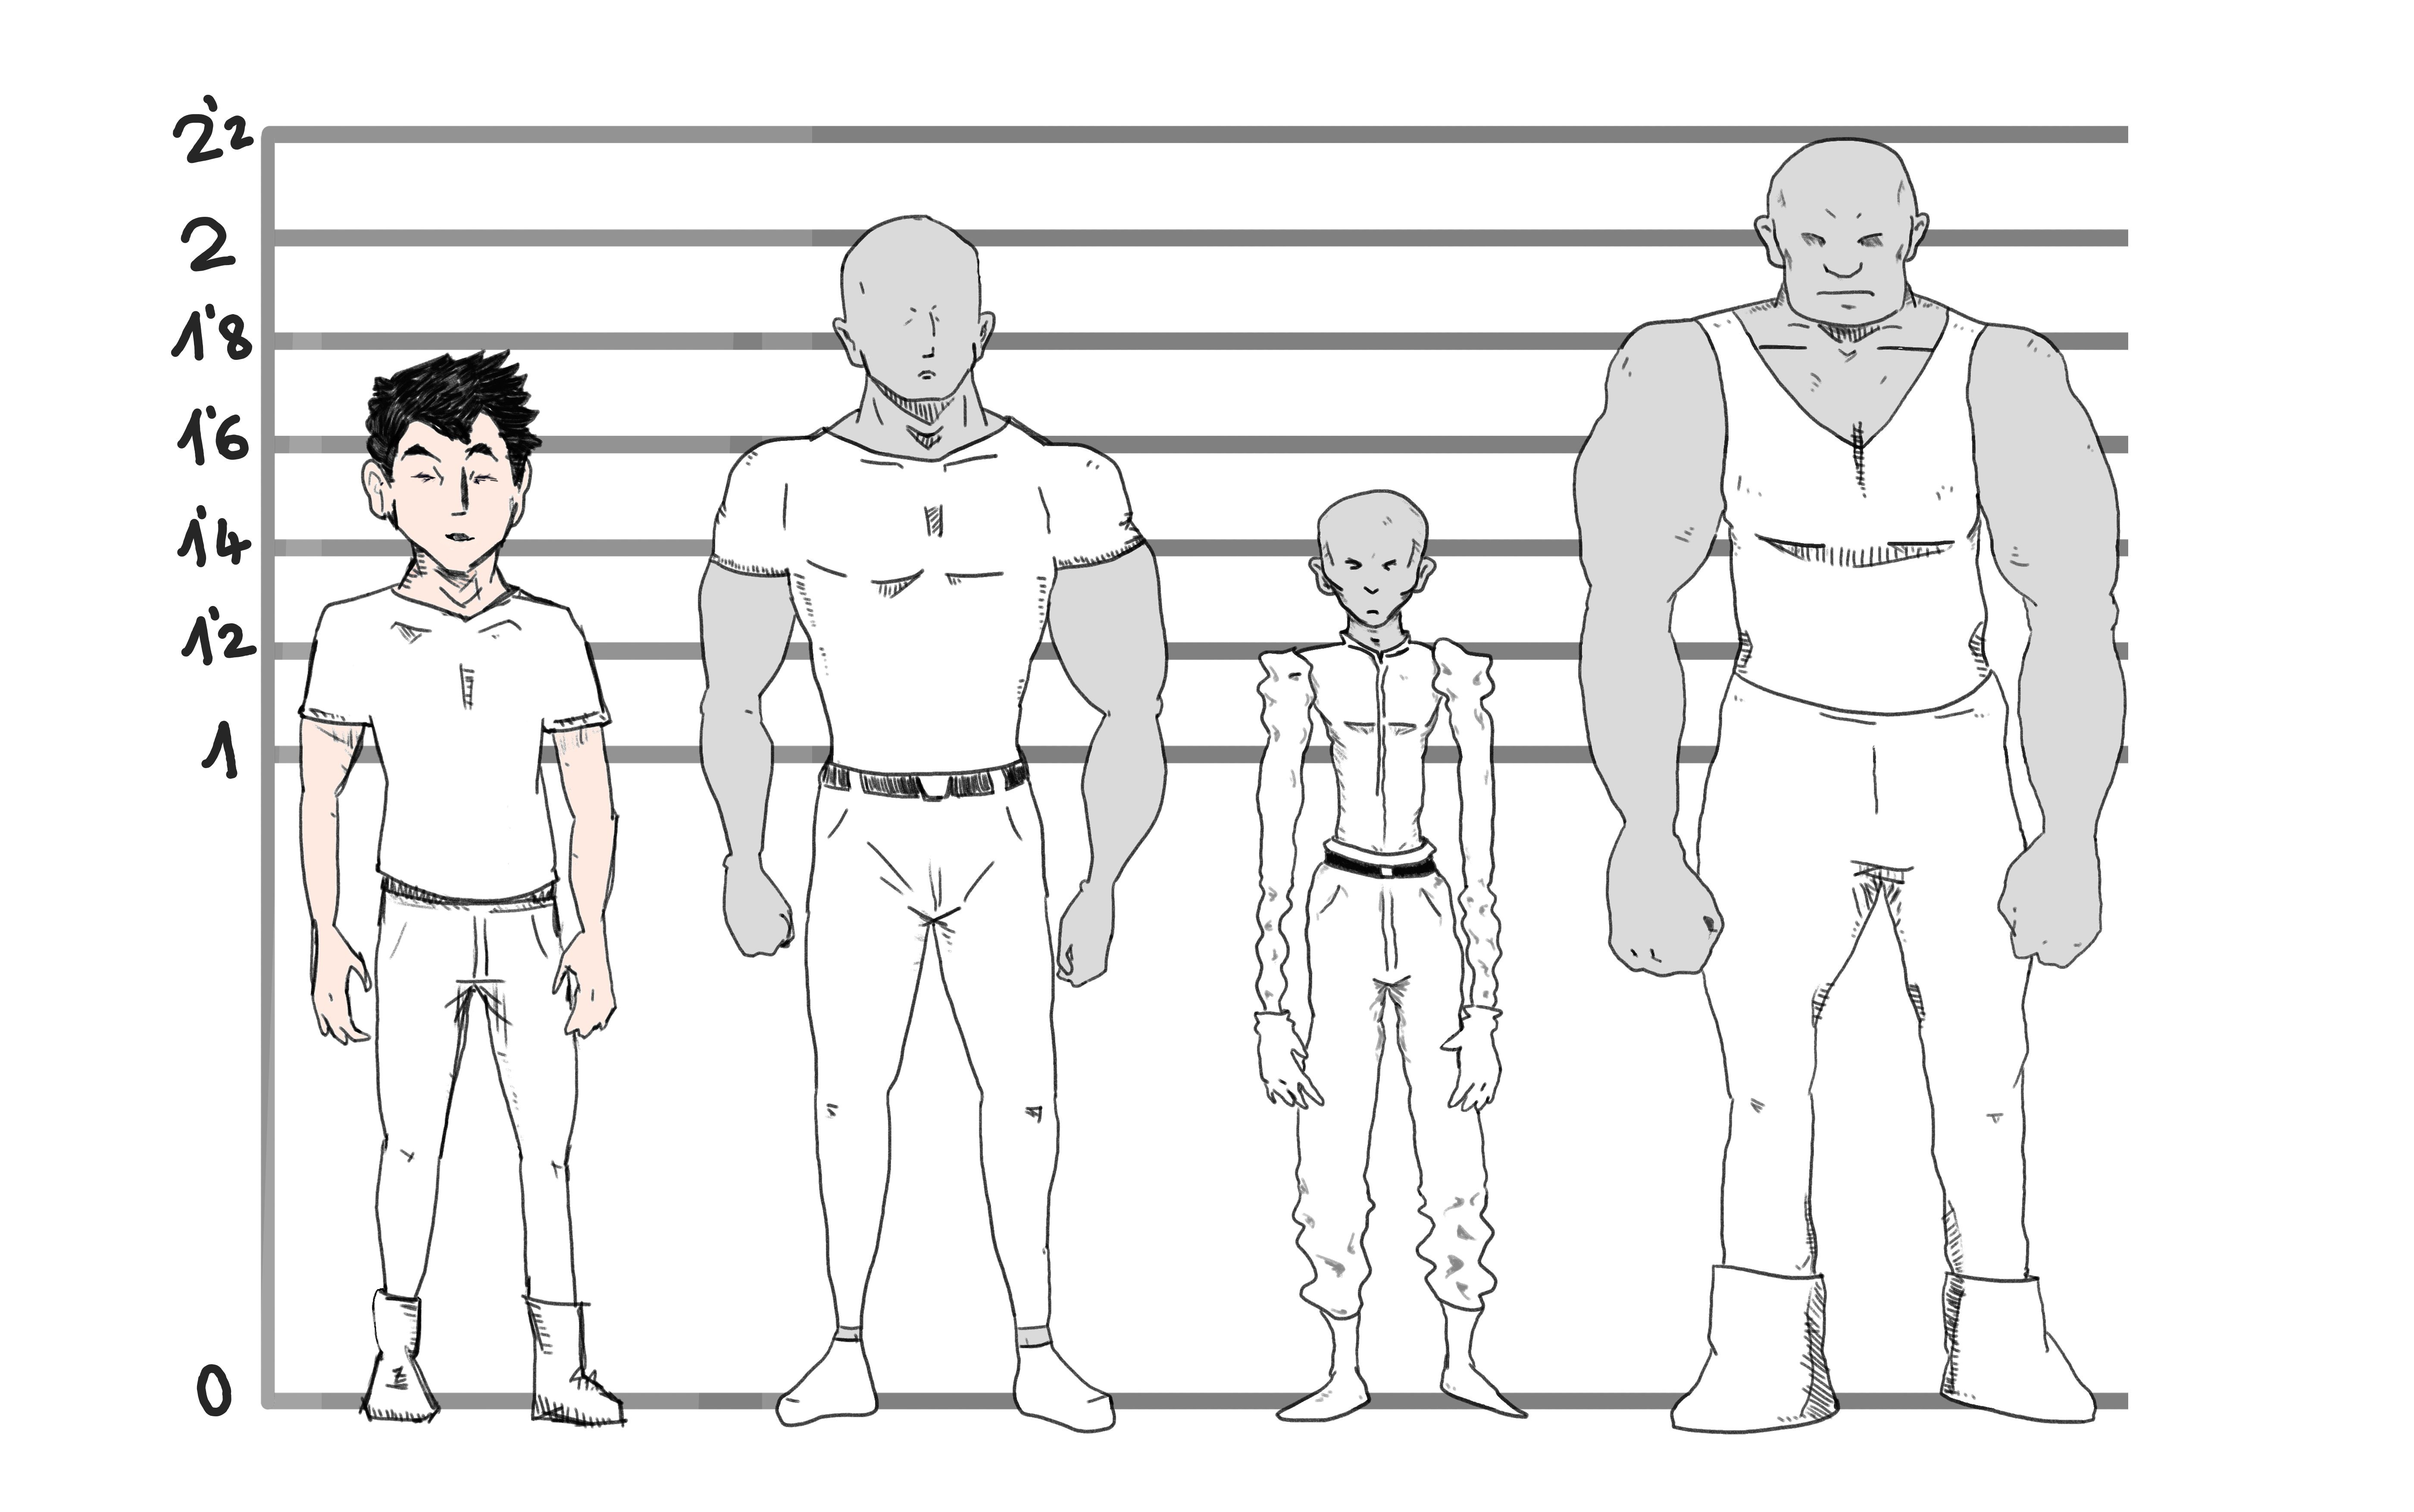
\includegraphics[width=0.75\textwidth]{images/races}}
      \newline{}Humanoide Rassen
      \label{fig:humanoide-rassen}
\end{figure*}
    

Im folgenden die relevanten Menschen und Mutantentypen.

\begin{description}
\item [Norms] Normal gebohrene Menschen werden Norms genannt. Seit der Besiedelung des Weltalls spielen die
      menschlichen Rassen keine so gro\3e Rolle mehr.
\item [Pure] Pure sind k"unstlich befruchtete, genetisch verbesserte Menschen. Das genetische Material wird vor der
      Befruchtung von negativen Genomen gereinigt. Pures sind Kinder der Superreichen und bilden einen signifikanten Teil der Oberschicht.
\item [Spacer] Spacer sind Humanoide, die ihr ganzes Leben in der Schwerelosigkeit verbracht haben. Bei Spacern haben
      sich Knochenmaterial und Muskel soweit zur"uck gebildet, dass sie sich nicht mehr ohne Exoskelett unter Schwerkraft wie auf der Erde oder dem Mars bewegen k"onnen. Stattdessen sind Spacer extrem geschickt in der Fortbewegung ohne Schwerkraft.
\item [Slags] Slags werden durch Strahlung mi\3gebildete Menschen genannt. Sie bilden den Bodensatz der
      humanen Gesellschaft.
\item [Alpha Mutant] Alphas sind die als Arbeiter in den extraterrestrischen Kolonien konzipierten Mutanten.
      Alphas sind deutlich kr"aftiger als Norms und haben einen deutlich stabileren und massigeren K"orperbau. Alphas haben eine gro\3e Resistenz gegen kosmische Strahlung und sind gut ger"ustet f"ur unterschiedliche Schwerkraftbedingungen. Alphas sind schwere Arbeit unter gef"ahrlichen Bedingungen gew"ohnt und haben meist einen gutm"utigen Charakter.
\item [Eta Mutant] Etas sind als Piloten und Personal f"ur Raumschiffe konzipiert. Sie sind nur 1,35 bis 1,50 Meter gro\3
      und drahtig. Optimiert f"ur Schwerkraftextreme und erh"ohte kosmische Strahlung sind sie f"ur den Einsatz auf Raumschiffen optimal angepasst.
\item [Omega Mutant] Omega Mutanten sind als Infanterist im Armeedienst gez"uchtet. Sie sind 1,90 bis 2,10 Meter gro\3.
      Omegas sind "ahlich wie Alphas extrem kr"aftig und haben eine nahezu unzerst"orbare Konstitution. Omegas sind von klein auf f"ur den Kampf ausgebildet, haben taktische Erfahrung und kennen den Umgang mit allen Waffensystemen.
\end{description}

\newsection{Technologie}

Ein Gro\3teil der Shadowrun-Regeln, Cyberware und die Matrix als Virtuelle Realit"at k"onnen "ubernommen werden.

Im folgenden ein kleiner Auszug aus den spezieller Technologie der 23.~Jahrhunderts. Ideen f"ur weitere Technologie k"onnen aus anderen near Future Rollenspielen wie Shadowrun, Cyberpunkt, Alien etc.~"ubernommen werden.

\begin{description}
\item [ComLink] Ein ComLink wird zur drahtlosen Verbindung in das ComNetz genutzt. Das ComLink ist entweder als
      Mobilger"at mit AR Brille oder als Headware verf"ugbar.
\item [ComNetz] Ein ComNetz ist auf den meisten menschlichen Siedlungen etabliert. Das ComNetz ist eine virtuelle
      Computerwelt und Kommunikationsinfrastruktur. In das ComNetz bindet man sich per ComLink ein. Per Augmented Reality (AR) werden Informationen und Steuerelemente in das audiovisuelle Zentrum der Teilnehmer eingeblendet. Das ComNetz wird f"ur die Kommunikation, zur Informationsbeschaffung, f"ur Finanztransfers, zur Steuerung von Ger"aten etc.~genutzt. Um tiefer in das Netz einzutauchen und in einer vollsensorischen Virtuellen Realit"at einzutauchen, wird eine kabelgebundene Verbindung "uber eine Datenbuchse ben"otigt.
\item [Commandchip] Der Commandchip ist die Ankopplungszentrale an das Gehirn. Der Commandchip erlaubt es Augmented Reality (AR) Signale in     das Sehzentrum und das H"ohrzentrum einzuspielen wie auch alle anderen Headware anzubinden.
\item [Credcard] Eine Credcard ist das Pendant zum ehemaligen Papiergeld. Eine vorher mit Geld aufgeladene Karte kann an
      einen Zahlungsempf"anger gegeben werden oder es kann per ComLink Geld von einer Credcard transferiert werden.
\item [Datenbuchse] Eine Datenbuchse ist eine am Hinterkopf verbaute Kabelschnittstelle zu einer Headware.
\item [Fusionstriebwerk] Fusionstriebwerke bilden den Hauptantrieb von Raumschiffen. "Uber Man"ovrierd"usen werden
      Raumschiffe in die richtige Positionen gebracht, um die m"achtigen Fusionstriebwerke zur Beschleunigung oder zum Abbremsen zu benutzen. Fusionstriebwerke nutzen eine Kernfusion mit HE-3 als Brennstoff und Wasser als Treibmasse.
\item [Headware] Mit dem Gehirn verbundene Hardware im Kopf, z.B.~ein ComLink das das ComNetz direkt mit dem Gehirn
      verbindet.
\item [ID--Chip] Menschen und Mutanten werden durch einen im linken Arm unter der Haut implantierten ID--Chip
      identifiziert. Der ID--Chip dient als Pass oder auch der Autorisierung von Zahlungen. Mittels Near--Field-Communication kann ein Reader auf den ID--Chip zugreifen.
\item [Magnetstiefel] Mangnetische Stiefel dienen dazu, in Schwerelosigkeit auf einem Raumschiff oder einer Station zu
      laufen. Zur Aktivierung werden sie zusammengeschlagen.
\item[PAN] Ein PAN (Personal Area Network) ist ein technisches System im Kopf der Person und umf"asst z.B.~ einen Commandchip und   
      die Anbindungen des Girns an weitere Cyberware im K"orper wie auch angebundene Systeme au\3erhalb des K"orpers.
\item [Psychonauten] Psynchonauten sind Personen, die "uber eine kabelgebundene Verbindung das Gehirn
      einer anderen Person infiltrieren k"onnen. Dieser Gehirnscan erlaubt es, Gedanken, Erinnerungen und Gef"uhle des anderen zu erforschen. Da es sich um eine bidirektionale Verbindung handelt, erf"ahrt auch der Gescante evtl.~etwas "uber den Psychonauten. Ein Gehirnscan ist gef"ahrlich und kann zum Gehirntot der gescanten Person f"uhren.
\item [Raumanzug] Im 23.~Jahrhundert haben sich Raumanz"uge zu Tauchanz"ugen "ahnlichen Bodysuites entwickelt, die unter
      normaler Kleidung getragen werden k"onnen. Raumanz"uge sch"utzen vor Druck und Temperaturunterschieden. Zusammen mit Druckluftkanistern und Gesichtsmasken erlauben sie den Aufenthalt in Weltall.
\item [Riggersteuerung] Eine Riggersteuerug erlaubt es technische Ger"ate fern zu steuern. Die Riggersteuerung wird direkt im 
      Gehirn verbaut und mit dem Commandchip verbunden oder extern "uber die Datenbuchse angebunden.
\item[Talentchip] Talentsoft erweitert den Tr"ager "uber den Commandchip um neue geistige und physische F"ahigkeiten. 
\end{description}

\newsection{Waffen}

Im folgenden ein Auszug von im 23.~Jahrhundert gebr"auchlichen Waffen.

\begin{description}
\item [Vibrokling] Eine durch hochfrequente Vibration extrem scharfe Klinge.
\item [Bolter] Ein Bolter ist eine semi automatische elektrisch getriebene Faustfeuerwaffe. Ein Bolter arbeitet "ublicherweise auf  
      dem Prinzip einer Railgun. Eine Railgun beschleunigt Hochgeschwindigkeitsprojektile entlang von zwei unter Strom gesetzten Stangen.
\item [Multigun] Eine Multigun in den meisten F"allen eine sehr gro\3e Faustfeuerwaffe ist eine Railgun die es erlaubt zwischen     
      penetrierenden Projektilen und Schockmunition umzuschalten.
\item [Railgun Gewehr] Ein Railgun Gewehr oder kurz eine Railgun ist eine vollautomatische langl"aufige Version einer nach 
      dem Railgun Prinzip funktionierenden Faustfeuerwaffe. Railguns werden auch auf Schiffen als Verteidigung gegen anfliegende Geschosse genutzt.         
\item [Plasmawerfer] Ein Plasmawerfer ist eine Infanteriewaffe, die von Omega-Mutanten in einem Kampfpanzer zusammen mit
      einem R"uckentornister getragen wird. Der Plasmawerfer verschie\3t hochenergetisches Plasma, das nahezu alles au\3er schweren Stahlplatten verbrennen kann.
\item [Raketenwerfer] Raketenwerfer sind eine der Hauptwaffensysteme von Raumschiffen.      
\item [Gefechtspanzer] Ein Gefechtspanzer ist ein Exoskelett mit starker Panzerung, eingebautem Raumanzug, Sensorik,
      Waffenplattformen und einem Jetpack. Ein Gefechtspanzer wird von Omega-Infanteristen eingesetzt.
\item [Gau\3kanone] Eine Gau\3kanone ist eine Waffensystem das auf Raumschiffen zum Einsatz kommt. "Uber mehrere Spulen
      werden Projektile in einem elektrisches Feld beschleunigt. Eine Gau\3kanone verschie\3t mit hoher Feuerrate Hochgeschwindigkeitsprojektile und gilt als die durchschlagskr"aftigste Feuerwaffe im Sonnensystem.         
\end{description}

\begin{figure*}[htbp]
      \centering
      \fbox{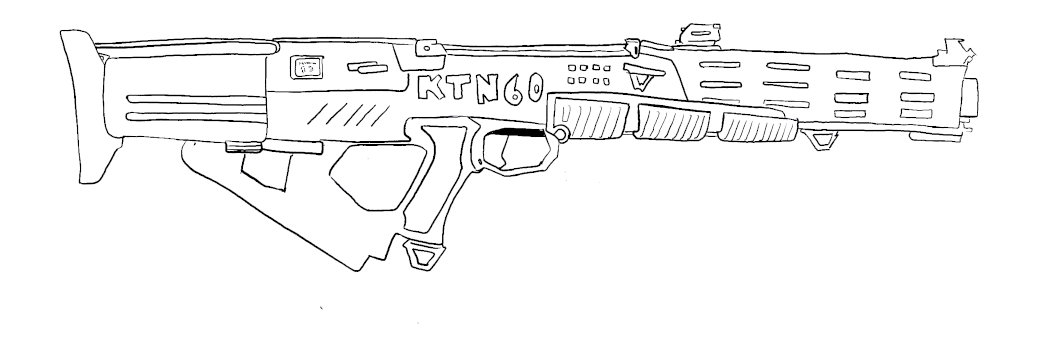
\includegraphics[width=0.75\textwidth]{images/guns}}
      \newline{}Railgun
      \label{fig:rail-gun}
\end{figure*}

\newsection{Kommunikation}

Das jovianische System besitzt erst nach der Besiedelung durch das Protektorat eine nennenswerte Infrastruktur. Durch den rasanten Aufbau hat jedoch ein Gro\3teil der Einrichtungen einen provisorischen Charakter. Diese sind zudem auf das Notwendigste beschr"ankt. Das gilt auch f"ur die Kommunikations-- und Informationssysteme. Wo auf Erde und Mars ein gutes ComNetz jegliche Information an jedem Punkt im System bereit stellt, steht ein voll ausgebautes ComNetz hier nur in Konzernsektoren und beim Milit"ar bereit.

Im jovianischen System  betreiben die einzelnen Monde und Stationen meist ein autonomes Kommunikationssystem, das mit den anderen Siedelungen und Anlagen nur in Teilen integriert ist. Ein ComNetz ist nur zwischen Monden und Stationen der Cynarian Corporation eingerichtet. Alle weitere Kommunikation zwischen Monden und Stationen erfolgt über Einzelverbindungen mittels der Sateliten rund um den Jupiter. Diese Verbindungen erlauben nur Kommunikation und Nachrichten zwischen Personen. Da die Stationen und Monde oft mehrere Millionen Kilometer voneinander entfernt sind, muss mit einer Kommunikationsverz"ogerung von mehreren Sekunden gerechnet werden.

Durch den steten unkontrollierten Zustrom von Mutantenfl"uchtlingen, Gl"ucksrittern und neuen Firmen stehen kaum Informationen zu Einzelpersonen und ans"assigen Institutionen und Unternehmen bereit.

\newsection{Fortbewegung und Reisezeiten}

Gro\3e Unternehmen wie Cynarian, das Protektoratsmilit"ar und die Protektoratsadministration betreiben eigene Shuttleflotten innerhalb des Systems soweit n"otig. Einige wenige Personen besitzen ebenfalls Shuttles. Der Rest der Fl"uge zwischen den Jupitertrabanten wird durch Transportunternehmen und Schiffseignern von Shuttles bereitgestellt. Einen Flug bekommt man am einfachsten im Raumhafen der jeweiligen Station. Da die Entfernungen im Jupterystem oft enorm sind sind Reisezeiten von 1 bis 2 Wochen bei zivilen Schiffen "ublich.
